\documentclass[a4paper,12pt]{article}
\usepackage[utf8]{inputenc}
\usepackage[russian]{babel} 
\usepackage{graphicx} 
\usepackage{amsmath}
\usepackage{amssymb}
\usepackage{float}
\usepackage[colorlinks=true, linkcolor=blue]{hyperref}
\usepackage{enumitem}

\renewcommand{\floatpagefraction}{0.99}
\renewcommand{\topfraction}{0.99}      

\title{ Задача со стержнем}
\author{Ларионов Станислав Александрович\and Доре Чойган Начын оглу \and Батанин Артём Александрович}
\date{\today}


\begin{document}

\maketitle

\newpage
\tableofcontents    
\newpage            


\section{Задача}
Объяснить физическую природу изменения слышимых частот вибраций алюмминивого стержня



\section{Теоретическое предположение}
В момент удара по стержню на его краю формируется очень крутой (почти прямоугольный) фронт сжатия. Такой резкий фронт сжатия порождает в стержне сразу ряд гармоник.
Эти гармоники можно получить если этот фронт разложить в ряд Фурье.

\begin{figure}[h!]
\centering
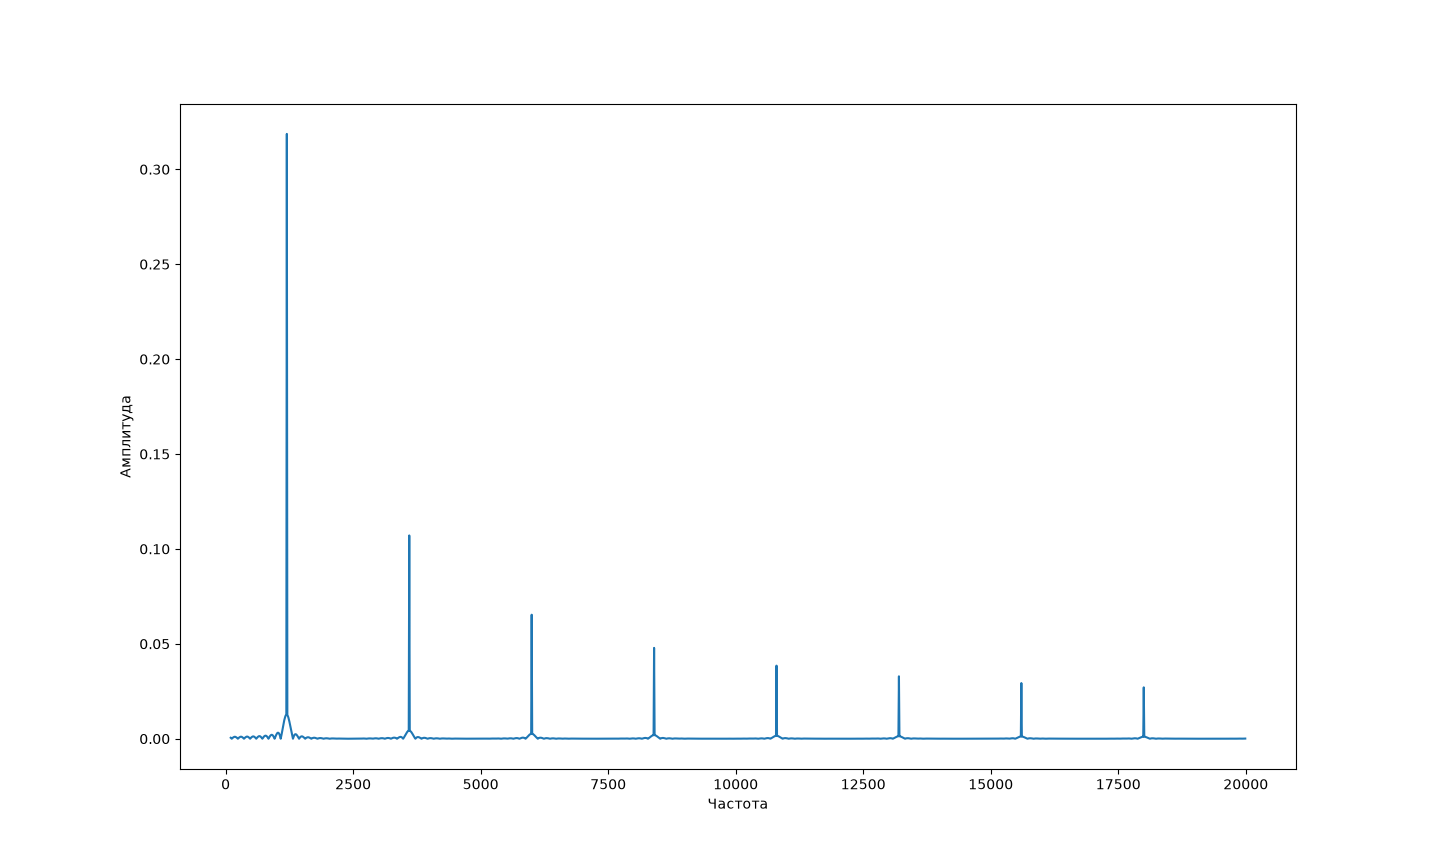
\includegraphics[width=0.5\linewidth]{media/Meandr.png}
\label{fig:meandr}
\caption{Пример разложения в ряд Фурье произвольного прямоугольного фронта}
\end{figure}

Стержень имеет набор резонансных частот - такие частоты, что половина длины волны целое число раз укладывается в длине стержня
Колебания, происходящие на частотах наиболее близких к резонансной частоте стержня имеют наибольшую добротность. Через некоторое время остаются только колебания с частотами наиболее близкими к резонансной или кратных ей частотам. 
Оценочная резонансная частота для метрового алюминиевого стержня - 3000Гц.



\section{Оценка спектра частот стержня}
Для изучения динамики изменения амплитуд, звуковые данные были разбиты на отрезки по 250мс, для каждого из которых рассчитывалось дискретное преобразование Фурье от 2кГц до 20 кГц (данные были записаны со стандартной частотой дискретизации аудио в телефоне -  48 кГц).  
В начальный момент времени видно около десятка различных пиков излучения ( Рис. \ref{fig:spektr}).
 
\begin{figure}[h!]
\centering
\includegraphics[width=1\linewidth]{media/1/gr/0_250.png}
\caption{Спектр излучения на промежутке от 0 до 250 мс}
\label{fig:spektr}
\end{figure}

Далее заметно, что меньше всего затухают колебания с частотами близкими или кратными 2840 Гц. (Рис. \ref{fig:spe}, Рис. \ref{fig:spektr3}, Рис. \ref{fig:spektr5}, Рис. \ref{fig:spektr6}, Рис. \ref{fig:spektr7}, Рис. \ref{fig:spektr8}, Рис. \ref{fig:spektr9}, Рис. \ref{fig:spektr10}, Рис. \ref{fig:spektr11}, Рис. \ref{fig:spektr12}, Рис. \ref{fig:spektr13})
На Рис. \ref{fig:spektr9} отчётливо видно, что оставшиеся пики - 2840гц 5680 и 11360 - колебания с кратными частотами, что подтверждает гипотезу резонанса 

\begin{figure}[H]
\centering
\includegraphics[width=1\linewidth]{media/1/gr/500_750.png}
\caption{Спектр излучения на промежутке от 500 до 750 мс}
\label{fig:spe}
\end{figure}


\begin{figure}[H]
\centering
\includegraphics[width=1\linewidth]{media/1/gr/1000_1250.png}
\caption{Спектр излучения на промежутке от 1000 до 1250 мс}
\label{fig:spektr3}
\end{figure}



%media/1/QR.png




\section{Вклады авторов}

Доре Чойган - оформление LaTex
Ларионов Станислав - анализ физической природы
Батанин Артём - написание кода, анализ данных

\newpage

\section{Ссылки на ресурсы}
Звуковые файлы с эксперимента лежат в папке media (sound.wav).
Данные анализа первого  удара (спектры с шагом в 250мс) и вырезанная аудиодорожка лежит в подпапке 1. 



\begin{figure}[H]
\centering

\includegraphics[width=1\linewidth]{media/1/QR.png}
\caption{Ссылка на репозиторий github}
\end{figure}







\newpage

\section{Графики спектров}

\begin{figure}[h!]
\centering
\includegraphics[width=1\linewidth]{media/1/gr/0_250.png}
\caption{Спектр излучения на промежутке от 0 до 250 мс}
\label{fig:spektr5}
\end{figure}





\begin{figure}[h!]
\centering
\includegraphics[width=1\linewidth]{media/1/gr/250_500.png}
\caption{Спектр излучения на промежутке от 250 до 500 мс}
\label{fig:spektr6}
\end{figure}



\begin{figure}[h!]
\centering
\includegraphics[width=1\linewidth]{media/1/gr/750_1000.png}
\caption{Спектр излучения на промежутке от 750 до 1000 мс}
\label{fig:spektr7}
\end{figure}


\begin{figure}[h!]
\centering
\includegraphics[width=1\linewidth]{media/1/gr/1750_2000.png}
\caption{Спектр излучения на промежутке от 1750 до 2000 мс}
\label{fig:spektr8}
\end{figure}


\begin{figure}[h!]
\centering
\includegraphics[width=1\linewidth]{media/1/gr/2250_2500.png}
\caption{Спектр излучения на промежутке от 2250 до 2500 мс}
\label{fig:spektr9}
\end{figure}

\begin{figure}[h!]
\centering
\includegraphics[width=1\linewidth]{media/1/gr/3000_3250.png}
\caption{Спектр излучения на промежутке от 3000 до 3250 мс}
\label{fig:spektr10}
\end{figure}


\begin{figure}[h!]
\centering
\includegraphics[width=1\linewidth]{media/1/gr/5250_5500.png}
\caption{Спектр излучения на промежутке от 5250 до 5500 мс}
\label{fig:spektr11}
\end{figure}

\begin{figure}[h!]
\centering
\includegraphics[width=1\linewidth]{media/1/gr/7500_7750.png}
\caption{Спектр излучения на промежутке от 7500 до 7750 мс}
\label{fig:spektr12}
\end{figure}

\begin{figure}[h!]
\centering
\includegraphics[width=1\linewidth]{media/1/gr/8250_8500.png}
\caption{Спектр излучения на промежутке от 8250 до 8500 мс}
\label{fig:spektr13}
\end{figure}


\end{document}